\chapter{Hardware}
This chapter describes the basic concept and configuration of the car-system's hardware. A basic knowledge of Altera Quartus II is assumed. This chapter only describes the hardware configuration of the central FPGA, since the DE0-nano boards have been configured by the previous years group.
\section{Topology}
To keep the system as modular as possible, every task needed to control the car\footnote{here communication and car-control, not every thread} has it's own nios2-core. The cores communicate with each other using a share memory area of the onchip memory. The memory access is controlled by a hardware-mutex. Beside the share memory, every core has it's own memory. The control-core uses onchip memory for this, while the communication core has to use the SDRAM on the board, because the code will not fit on the limited space of the onchip memory. For communication with the other components of the car as well as the car2x communication, the responsible communication core uses one of the board's ethernet controllers. For programming and debugging purposes, both cores are accessable through a JTAG-UART. The topology is shown in figure \ref{HWtopo}.


\begin{center}
\begin{figure}[h]
	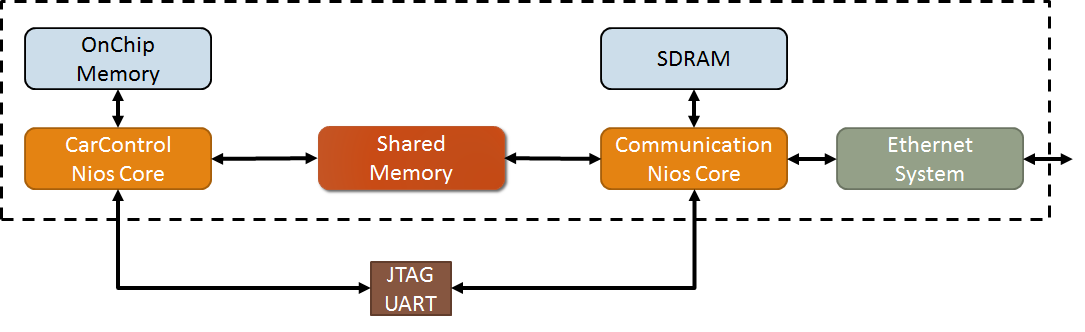
\includegraphics[width=\textwidth]{figures/FPGA_QSYS_Structure.png}
	\caption{Schematic hardware structure} \label{HWtopo}
\end{figure}
\end{center}

\section{Configuration QSYS}
The major part of the hardware configuration is done in the QSYS tool from altera. This projects configuration has been created using couple of altera tutorials and combining them. The part used for the ethernet configuration has been placed in a seperated QSYS file to clean up the configuration slightly. 

\section{Configuration Top Level File}
The top level files combines all subcomponents need to compile the system. This also connects the components, e.g. the QSYS-generated file with the in and output ports of the FPGA as well as additional components used by the ethernet of SDRAM controller. 

\section{Problems}
Probably the greatest problem where the altera tutorials, since they are designed to fulfil only the one task and combination or integration into a bigger system is not supported or described. For example the system clock needed for the ethernet controller to work is higher then the clock used in the sdram tutorial. And since the tutorials should be kept easy, a prebuild component is used with a hardcoded clock in it, which leads to timing problems and system crashes. Also the explanations in the tutorial, especially regarding the top-level file are kept to a minimum, by providing code to be copy-pasted.\\
Also due to timing problems it seems not to be possible to use one block of sdram for both cores. For that reason the control core still uses onchip memory.\\
Another problem was the limited debugging. The debugging function of eclipse is not working at all and the default console also sometimes produces errors. To bypass this, disabling the eclipse default console output is a good idea and using the nios2-terminal instead. This also allows debug outputs from both cores simultaneously. Because of this limited debug possibilities, it was quite hard to find if the error came from hardware or software, or even from a broken board/malfunctioning hardware.

\section{WiPort}
Paul - done

\section{Circuit diagrams}
Johannes
